\chapter{Hermite polynomials}
\label{h:hermite}

\begin{quote}
We are servants rather than masters in mathematics.

--- Charles Hermite
\end{quote}

\chaptertoc

In this chapter, we will look at Hermite polynomials, which are an example of a family of so-called orthogonal polynomials. They appear in the higher-order solutions of the paraxial wave equation.

After presenting the corresponding differential equation, we introduce their generating function and look at integrals involving these polynomials. We will also derive their orthogonality, as well as use them in series expansions.

\pagebreak

\sectionugent{The paraxial wave equation}

Wave propagation is governed by the Helmholtz equation:

\begin{equation}
\nabla^2 \psi({\mathbf r}) + k^2 \psi({\mathbf r}) = 0
\end{equation}

The paraxial wave equation is an approximation to the Helmholtz equation under the so--called slowly varying envelope approximation (SVEA). This approximation looks for solutions which are essentially plane waves propagating along the $z$--direction, but which are modulated by a slowly varying function $A({\mathbf r})$:

\begin{equation}
\psi({\mathbf r}) = A({\mathbf r})e^{-jkz}
\label{eq-svea-ansatz}
\end{equation}

This is typically done when studying systems which have a well-defined optical axis, along which most of the light is propagating, like in a lens system.

\begin{cue}
Calculate $\partial \psi^2 / \partial z^2$.
\end{cue}

For the first derivative, we get

\begin{equation}
\frac{\partial \psi({\mathbf r})}{\partial z} = \frac {\partial A({\mathbf r})}{\partial z}e^{-jkz} -j k A({\mathbf r})e^{-jkz}
\end{equation} 

This means that

\begin{equation}
  \frac{\partial^2 \psi({\mathbf r})}{\partial z^2} = \frac{\partial^2 A({\mathbf r})}{\partial z^2}e^{-jkz} - 2 j k \frac{\partial A({\mathbf r})}{\partial z}e^{-jkz} - k^2 A({\mathbf r})e^{-jkz}
 \label{eq-svea-d2} 
\end{equation} 

\begin{cue}
If $A({\mathbf r})$ varies slowly as a function of $z$, what does that mean? Obviously, $\partial A / \partial z$ should be small, but small with respect to what? Make sure you compare against something with the correct dimensions.
\end{cue}

You might be tempted to write down that

\begin{equation}
 \left|\partial A({\mathbf r}) / \partial z\right| \ll \left|A({\mathbf r})\right|
\end{equation} 

At least that way, the criterion is unaffected by multiplication of $A$ by an arbitrary scaling factor. However, the dimensions are wrong: on the right-hand side, we need to divide by something which has a dimension of meter. Using the wavelength as a yard stick for this seems like a good idea. Since dividing by $\lambda$ is equivalent to multiplying by the wavevector $k$, we get

\begin{equation}
\left|\partial A({\mathbf r}) / \partial z\right| \ll k \left|A({\mathbf r})\right|
\end{equation}

Taking the derivative with respect to $z$ once more, means we can neglect $\partial^2 A / \partial z^2$ with respect to $j k \partial A / \partial z$ in Eq~\ref{eq-svea-d2}.

\begin{cue}
Make this approximation and figure out what the Helmholtz equation reduces to.
\end{cue}

With this, the Helmholtz equation becomes

\begin{equation}
\fbox{$\displaystyle
\nabla_T^2 A({\mathbf r}) -2jk \frac{\partial A({\mathbf r})}{\partial z} = 0
$}
\label{eq-paraxial}
\end{equation} 

Here, $\nabla_T^2$ stands for the transverse part $(\partial^2 / \partial x^2) + (\partial^2 / \partial y^2)$ of the Laplacian operator.

\begin{marginfigure}[-5cm]
% credits: Wikipedia
% url: https://en.wikipedia.org/wiki/Carl_Friedrich_Gauss
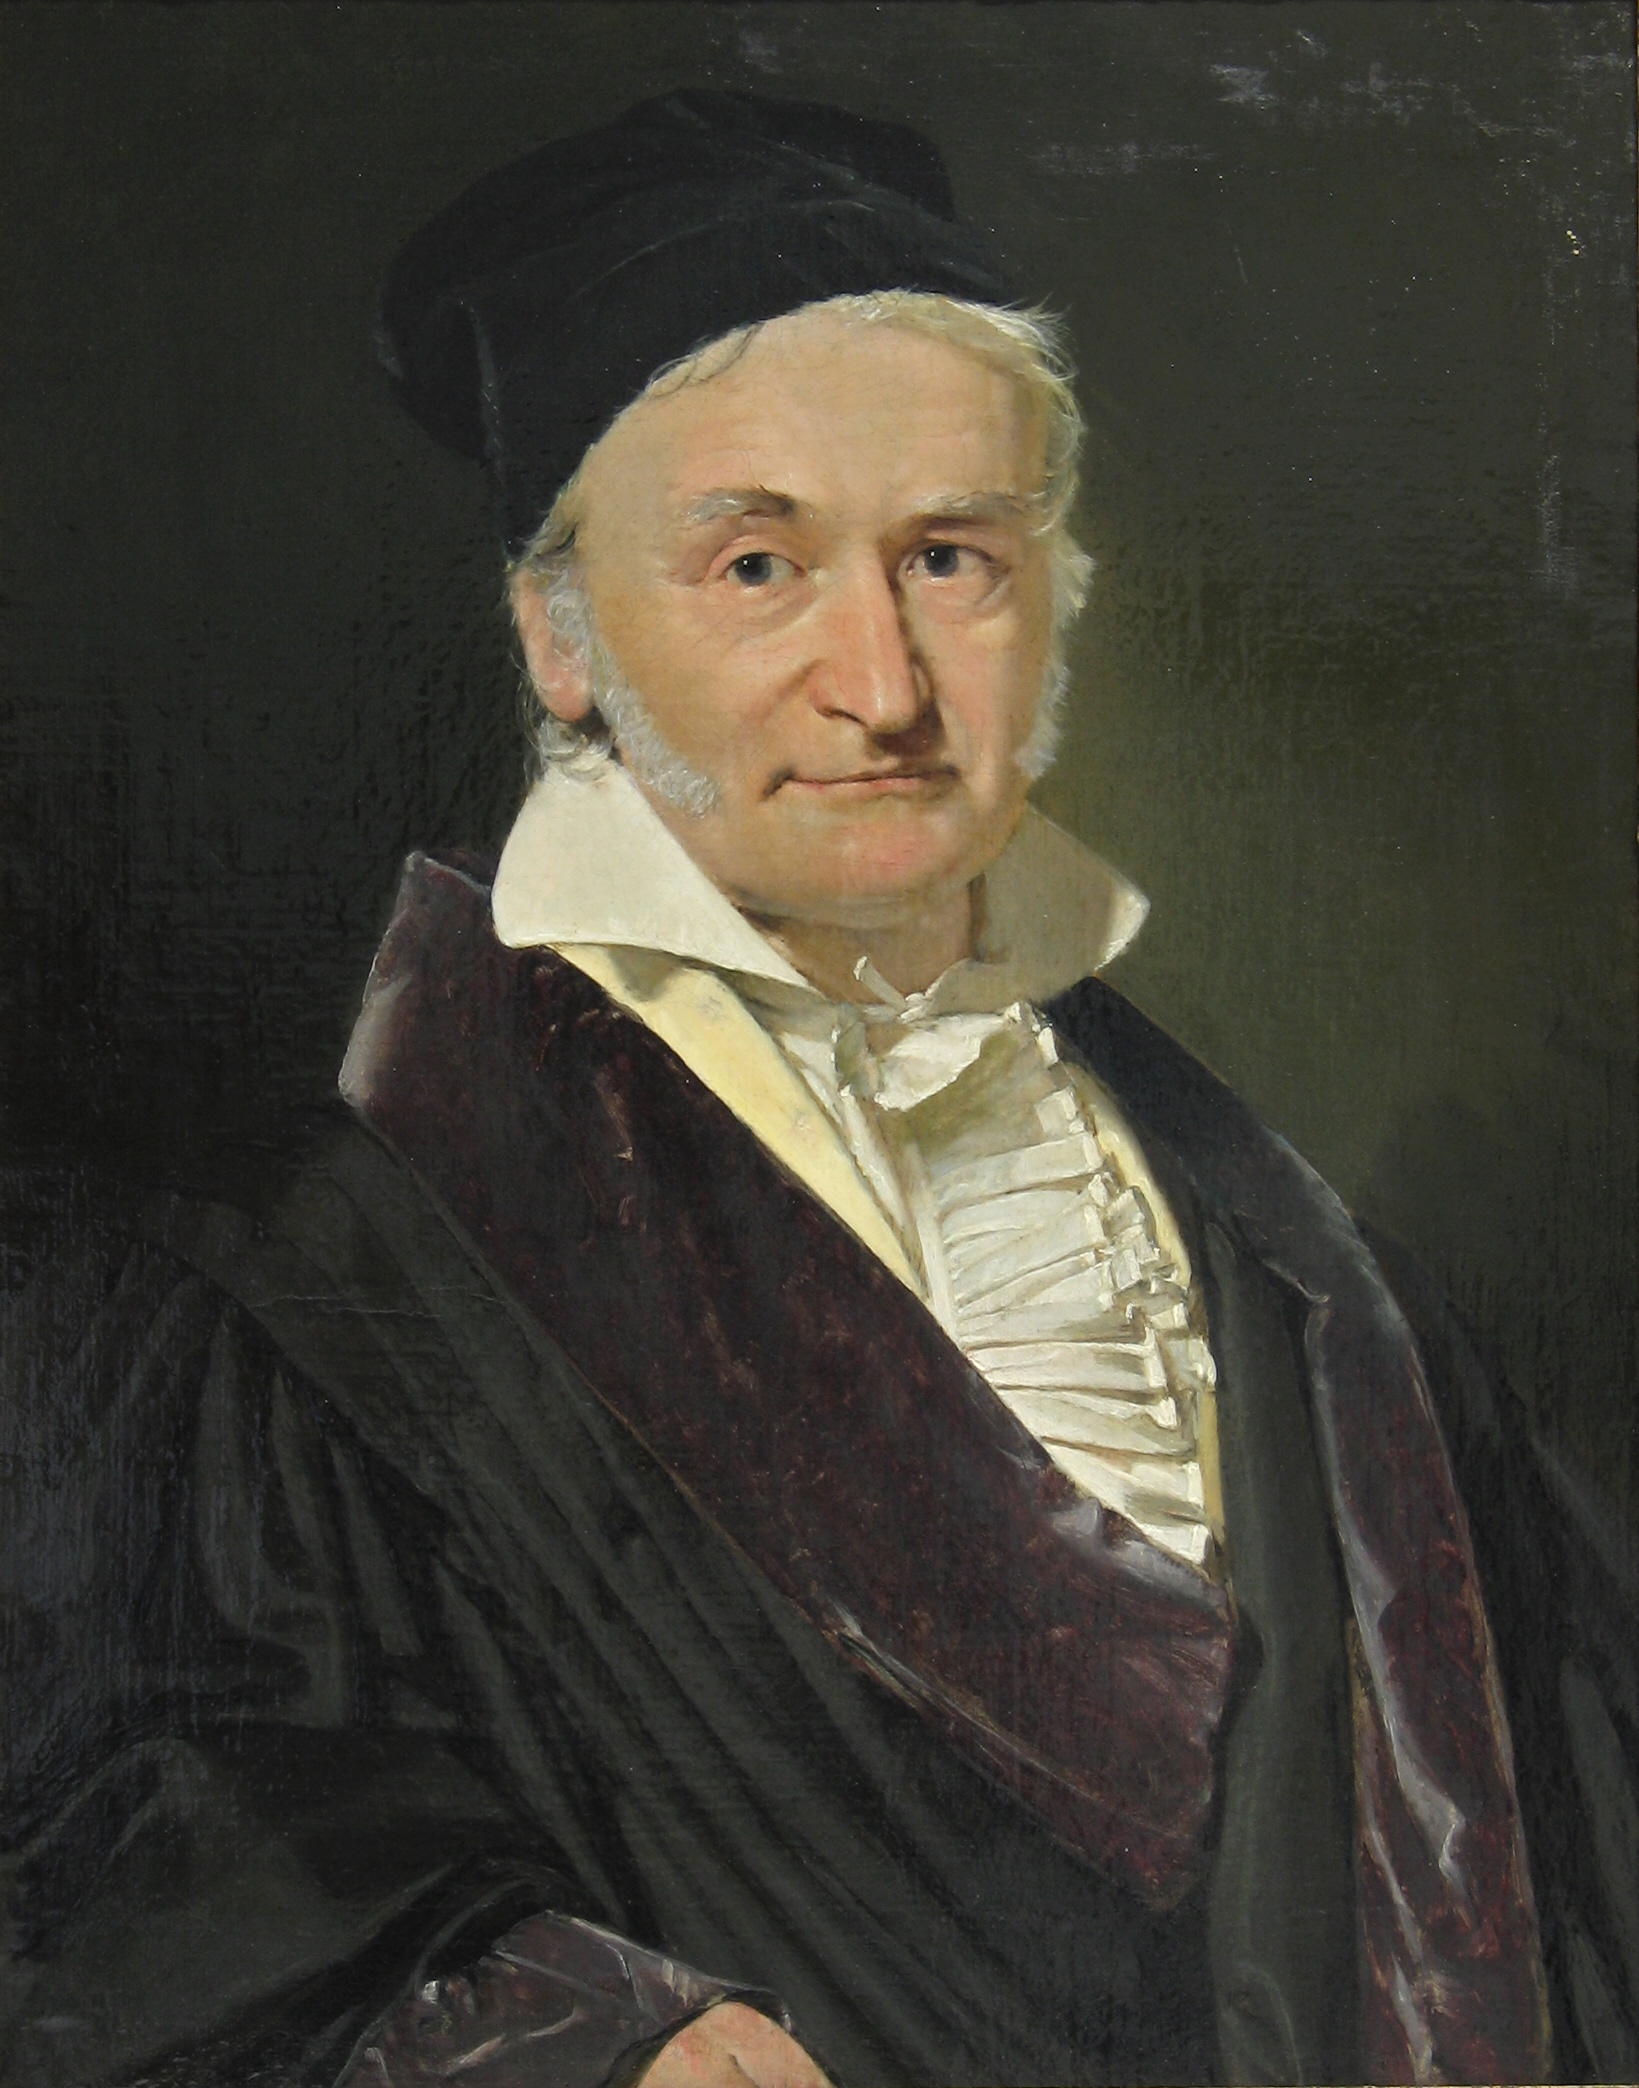
\includegraphics{hermite/figures/c_gauss}
\caption{Carl Friedrich Gauss (1777-1855)}
\end{marginfigure}

It is possible to show that a solution to this equation is the following function, which describes a so-called Gaussian beam:

\begin{equation}
A_G({\mathbf r}) = \frac{1}{q(z)}e^{-\frac{jk\rho^2}{2q(z)}} \label{eq-gauss}
\end{equation}   

where $q(z)=z+jb_0$. 

In this context, the function $W(z)$ is defined as

\begin{equation}
W(z)=\sqrt{\frac{2 b_0}{k} \left(1 + \frac{z^2}{b_0^2}\right)} \label{eq-W}
\end{equation} 

$W(z)$ can be interpreted as the width of the Gaussian beam.


\pagebreak


\section{Hermite's differential equation}

Let's look for higher-order solutions to the paraxial wave equation. To achieve this, let's try a modulated version of the Gaussian beam:

\begin{equation}
A(x,y,z) = X\left({\frac{\sqrt{2}x}{W(z)}}\right) Y\left({\frac{\sqrt{2}y}{W(z)}}\right) e^{-jZ(z)} A_G(x,y,z) \label{eq-gauss-higher}
\end{equation} 

Here, $A_G$ is the Gaussian beam from Eq.~\ref{eq-gauss} and $X()$, $Y()$ and $Z()$ are three real--valued functions that we still need to determine such that Eq.~\ref{eq-gauss-higher} satisfies the paraxial Helmholtz equation.

\begin{cue}
Calculate $\partial A^2 / \partial x^2$. Use the definition of the Gaussian beam Eq.~\ref{eq-gauss}. 
\end{cue}
  
For the x--derivative of Eq.~\ref{eq-gauss-higher}, we get

\begin{equation}
\frac{\partial A}{\partial x} = \frac{\sqrt{2}}{W}X'Ye^{-jZ} A_G + XYe^{-jZ} \frac{\partial A_G}{\partial x} 
\end{equation} 

and

\begin{equation}
\frac{\partial^2 A}{\partial x^2} = \frac{2}{W^2}X''Ye^{-jZ} A_G  + 2\frac{\sqrt{2}}{W}X'Ye^{-jZ} \frac{\partial A_G}{\partial x}  + XYe^{-jZ} \frac{\partial^2 A_G}{\partial x^2}
\end{equation} 

Or, using Eq.~\ref{eq-gauss} to calculate $\partial A_G / \partial x$:

\begin{equation}
\frac{\partial^2 A}{\partial x^2} = \frac{2}{W^2}X''Ye^{-jZ} A_G  - 2j k x \frac{\sqrt{2}}{qW}X'Ye^{-jZ}A_G  + XYe^{-jZ} \frac{\partial^2 A_G}{\partial x^2} \label{eq-hermite-gauss-1}
\end{equation} 

We can derive a similar equation for the $y$--derivative.

\begin{cue}
Calculate $\partial A / \partial z$. Use the definition of the Gaussian beam Eq.~\ref{eq-gauss}. 
\end{cue}

For the $z$--derivative, we get

\begin{align}
\frac{\partial A}{\partial z} =  -\frac{\sqrt{2}x W'}{W^2}X'Ye^{-jZ} A_G -\frac{\sqrt{2}y W'}{W^2}XY'e^{-jZ} A_G \nonumber \\ 
+ XY\left(-jZ'\right)e^{-jZ} A_G + XYe^{-jZ}\frac{\partial A_G}{\partial z} \label{eq-hermite-gauss-2}
\end{align} 

\begin{cue}
Plug these results into the paraxial wave equation and divide by $XY$.
\end{cue}

Let's substitute this in the paraxial equation Eq.~\ref{eq-paraxial}. Because $A_G$ is itself a solution of this equation, the last terms from Eq.~\ref{eq-hermite-gauss-1} and \ref{eq-hermite-gauss-2} cancel and we get:

\begin{align}
\frac{2}{W^2}\left(X''Y+XY''\right)e^{-jZ} A_G  \nonumber \\
-2jk \frac{\sqrt{2}}{Wq}\left(xX'Y+yXY'\right)e^{-jZ}A_G \nonumber \\
+2jk \frac{\sqrt{2} W'}{W^2}\left(xX'Y+yXY'\right)e^{-jZ}A_G \nonumber \\
-2jk XY\left(-jZ'\right)e^{-jZ} A_G = 0
\end{align}

Getting rid of the common factors and dividing by $XY$, we get

\begin{equation}
\frac{1}{W^2}\left(\frac{X''}{X}+\frac{Y''}{Y}\right)  
- j k \left(\frac{\sqrt{2}}{Wq} - \frac{\sqrt{2}W'}{W^2}\right)\left(x\frac{X'}{X}+y\frac{Y'}{Y}\right)
-kZ' = 0
\end{equation} 

or
\begin{equation}
\left(\frac{X''}{X}+\frac{Y''}{Y}\right)  
- j k  \left(\frac{W^2}{q} - W'W\right)\frac{\sqrt{2}}{W}\left(x\frac{X'}{X}+y\frac{Y'}{Y}\right)
-kW^2Z' = 0
\end{equation} 

\begin{cue}
Simplify $W^2/q - W'W$ and perform the change of variables $u = \sqrt{2} x / W(z)$ and  $v = \sqrt{2} y / W(z)$. Then, perform separation of variables for the resulting differential equation. 
\end{cue}

Using the definitions for $W$ and $q$, it follows that $W^2/q - W'W = -j \lambda / \pi$. If we now perform the change of variables $u = \sqrt{2} x / W(z)$ and  $v = \sqrt{2} y / W(z)$, we get

\begin{equation}
\left[{\frac{X''(u)}{X(u)} - 2 u\frac{X'(u)}{X(u)}}\right] + 
\left[{\frac{Y''(v)}{Y(v)} - 2 v\frac{Y'(v)}{Y(v)}}\right] -kW^2(z)Z'(z) = 0
\end{equation} 

The left--hand side of this equation is a sum a three terms, each of which is a function of a single independent variable ($u$, $v$ and $z$ respectively). Therefore, each of these terms must be equal to a constant. Equating the first term to $-2\mu_1$ and the second to $-2\mu_2$, the third must be equal to $2(\mu_1+\mu_2)$. This separation of variables leads to the following ordinary differential equations:

\begin{equation}
X''(u) - 2 u X'(u) = - 2 \mu_1 X(u) 
\end{equation} 

\begin{equation}
Y''(v) - 2 v Y'(v) = - 2 \mu_2 Y(v)
\end{equation} 

\begin{equation}
b_0\left(1 + \frac{z^2}{b_0^2}\right)Z'(z) = -(\mu_1+\mu_2)
\end{equation} 

From this, it follows immediately that $Z(z) = -(\mu_1+\mu_2) \arctan(z/b_0)$.

The differential equations for $X$ and $Y$ are both of the following form:

\begin{equation}
\fbox{$\displaystyle
X''(x) - 2 x X'(x) + 2 n X(x) = 0 \label{eq-diff-hermite-0}
$}
\end{equation} 

\begin{marginfigure}[-4.3cm]
% credits: Wikipedia
% url: https://en.wikipedia.org/wiki/Charles_Hermite
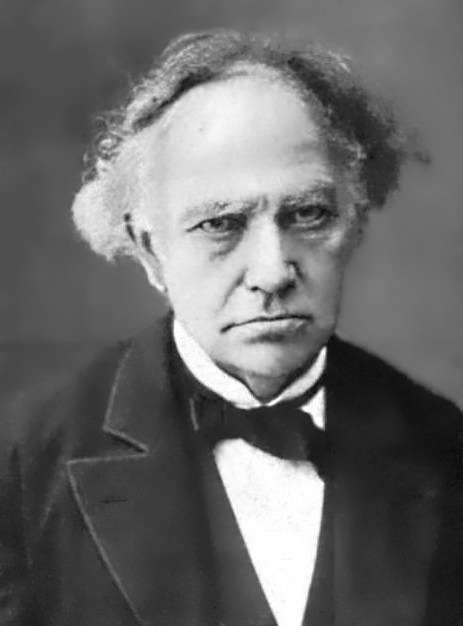
\includegraphics{hermite/figures/c_hermite}
\caption{Charles Hermite (1822–1901)}
\end{marginfigure}

They don't have any obvious solutions at first sight. In the next sections, we will show that their solutions are \emph{Hermite polynomials}, and that $n$ is an integer.

In a similar vein to the treatment of Bessel functions, we will start by introducing a generating function and then continue to derive recurrence relations which will lead to a differential equation.


\pagebreak


\sectionugent{Generating function for Hermite polynomials}

The generating function of the Hermite polynomials takes the following form:

\begin{equation}
g(x,t) = e^{-t^2 + 2tx} \label{eq-gen-hermite}
\end{equation}

The Hermite polynomials $H_n(x)$ are \emph{defined} from the the Laurent series in $t$ of $g(x,t)$ as 

\begin{equation}
\fbox{$\displaystyle
  g(x,t) = e^{-t^2 + 2tx} \stackrel{def}{=} \sum_{n = 0}^{\infty} H_n(x)\frac{t^n}{n!} \label{eq-g-hermite}
$}
\end{equation} 

\noindent\marginnote{An unfortunate side effect of the Latin alphabet having rather few letters...}Note the absence of a superscript in $H_n(x)$, which distinguishes them from the unrelated Hankel functions. The presence of $n!$ in the definition is purely cosmetic, and results in integer coefficients in the polynomial.

\begin{exer}
% difficulty: normal
% ugent
\noindent\marginnote[0.7cm]{See the solution video for a graphical representation of the different terms in the product.}Show that
$$H_n(x) = \sum_{r=0}^{\lfloor n/2 \rfloor}(-1)^r {(2x)}^{n-2r} \frac{n!}{(n-2r)! r!}$$
\end{exer}

With this formula, we can calculate the different polynomials (see Table~\ref{tab-hermite} and Fig.~\ref{fig-hermite}.)

\begin{figure}
\centering
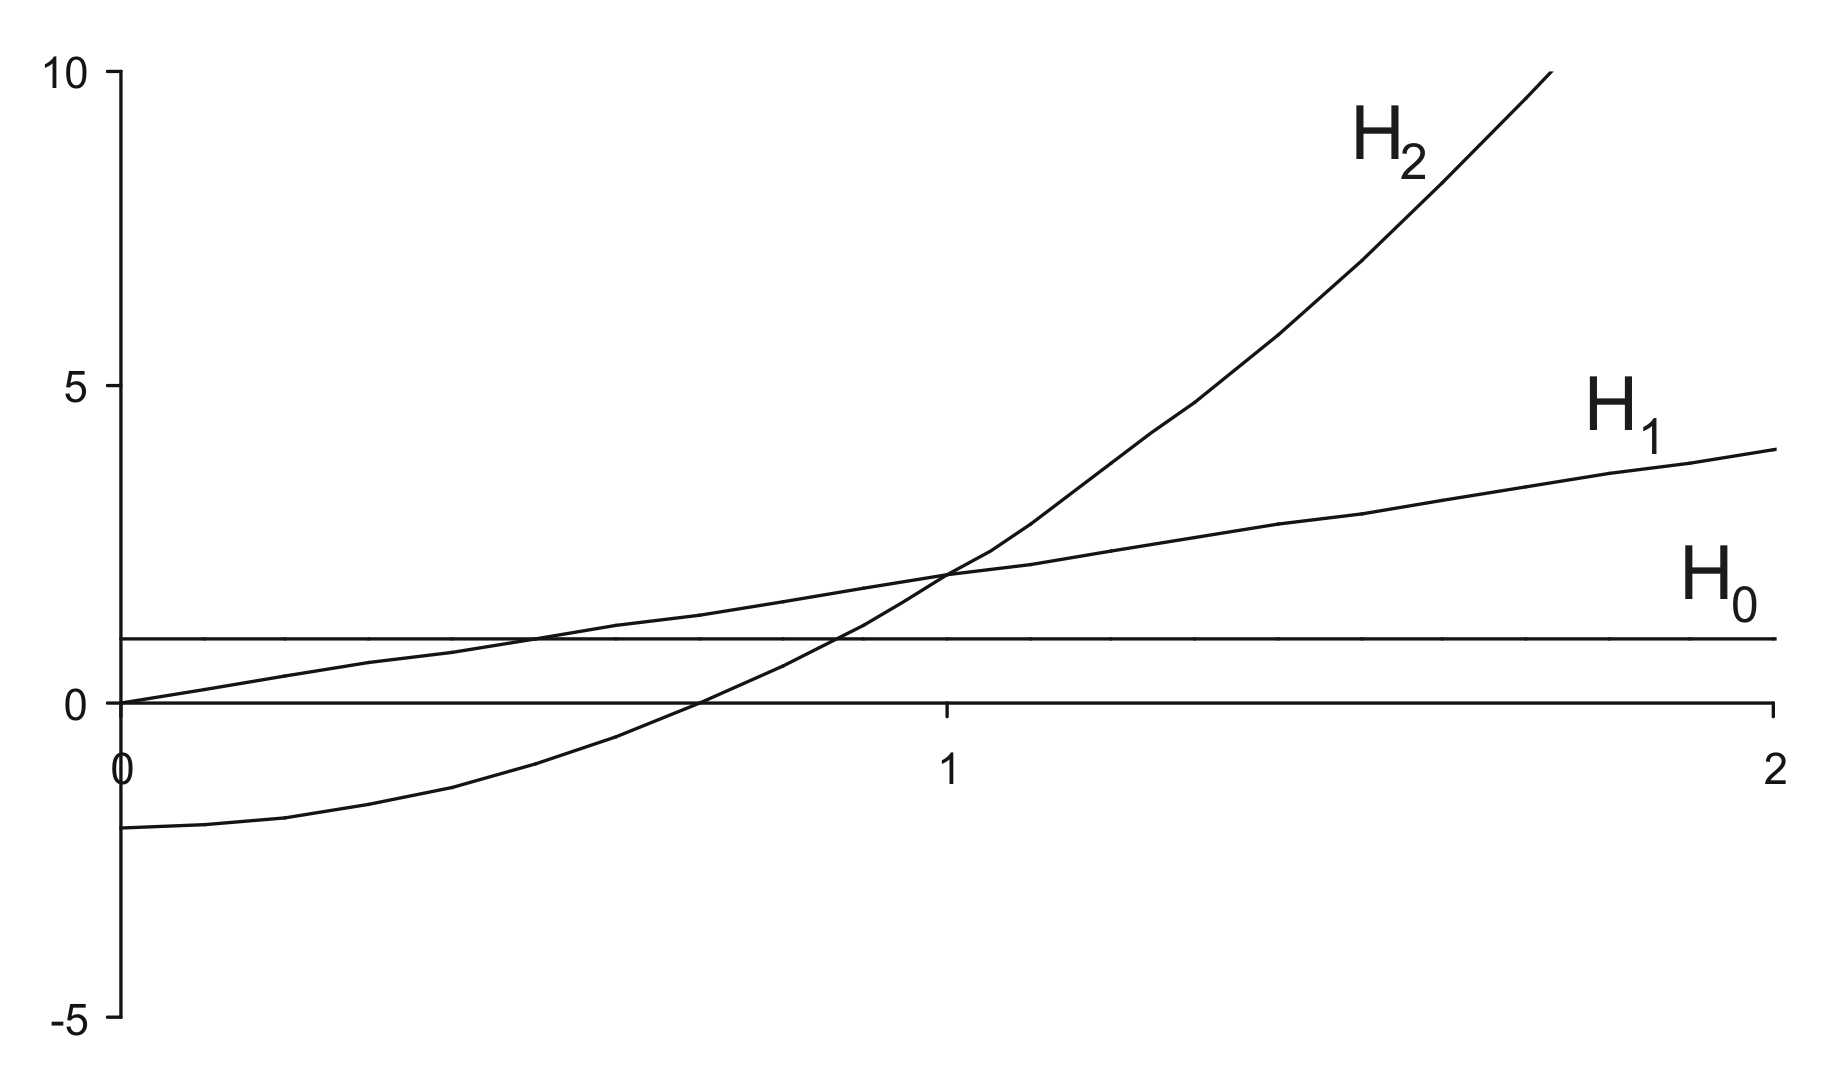
\includegraphics[scale=0.7]{hermite/figures/hermite}
\caption{The Hermite polynomials $H_0(x)$, $H_1(x)$, $H_2(x)$.}
\label{fig-hermite}
\end{figure}

\begin{table}
\begin{align}
H_0(x) = & \, 1 \nonumber \\
H_1(x) = & \, 2x \nonumber \\
H_2(x) = & \, 4x^2-2 \nonumber \\
H_3(x) = & \, 8x^3-12x \nonumber \\
H_4(x) = & \, 16x^4-48x^2+12 \nonumber \\
H_5(x) = & \, 32x^5-160x^3+120x \nonumber \\
H_6(x) = & \, 64x^6-480x^4+720x^2-120 \nonumber
\end{align}
\caption{Hermite polynomials}
\label{tab-hermite}
\end{table}

\pagebreak

\begin{exer}
% difficulty: normal
Compared to the generating function of the Bessel functions, what feature of the generating function of the Hermite polynomials makes that Hermite polynomials are actually polynomials, i.e. that their series expansion terminates?
\end{exer}

\begin{exer}
% difficulty: trivial
In Eq.~\ref{eq-g-hermite}, why are there no terms for negative powers of $t$?
\end{exer}

\begin{exer}
% difficulty: hard
Show that the coefficients of $H_n(x)$ are all integers.
\begin{hnt}
Factor out $n \choose r$.  
\end{hnt}
\end{exer}

\pagebreak


\sectionugent{Recurrence relations for Hermite polynomials}
\label{week5}

Similar to the treatment of Bessel functions, we can derive recurrence relations by differentiating the generating function.

\begin{cue}
By differentiating Eq.~\ref{eq-g-hermite} with respect to $t$ and derive a recurrence relation.
\end{cue}
 
By differentiating Eq.~\ref{eq-g-hermite} with respect to $t$, we get

\begin{equation}
(-2t+2x)e^{-t^2 + 2tx} = \sum_{n = 0}^{\infty} H_n(x) \frac{nt^{n-1}}{n!}
\end{equation} 

Substituting Eq.~\ref{eq-g-hermite} back in this, we get

\begin{equation}
(-2t+2x) \sum_{n = 0}^{\infty} H_n(x)\frac{t^n}{n!} = \sum_{n = 0}^{\infty} H_n(x) \frac{nt^{n-1}}{n!}
\end{equation} 

\noindent\marginnote{If you'd like more intermediate steps here, have a look at the video.}This leads to

\begin{equation}
-2  \frac{H_{n-1}(x)}{(n-1)!} + 2 x \frac{H_n(x)}{n!} = H_{n+1}(x) \frac{n+1}{(n+1)!}
\end{equation} 

where $n \geq 1$, or

\begin{equation}
H_{n+1}(x) = 2 x H_n(x) - 2 n H_{n-1}(x)
\label{eq-recur-hermite-1}
\end{equation} 
 

\begin{exer}
% difficulty: normal
% ugent
Show that
$$\displaystyle H_n'(x) = 2nH_{n-1}(x)$$ \label{eq-recur-hermite-2}
\end{exer}


\pagebreak


\sectionugent{Hermite's differential equation revisited}

Next step is showing that the polynomials as defined through the generating function satisfy Hermite's differential equation. We will do this using the recurrence relations we derived from the generating function.

\begin{cue}
Take the derivative of Eq.~\ref{eq-recur-hermite-1} with respect to $x$ and use the recurrence relationship involving $H_n'(x)$ to calculate  $H_{n+1}'(x)$ and $H_n''(x)$. Then, recover Hermite's differential equation.
\end{cue}

Differentiating Eq.~\ref{eq-recur-hermite-1} with respect to $x$, we get

\begin{equation}
H_{n+1}'(x) = 2  H_n(x) + 2 x H_n'(x)- 2 n H_{n-1}'(x)
\end{equation} 

Using the results from Ex. \ref{eq-recur-hermite-2}, we have $H_{n+1}'(x) = 2(n+1)H_n(x)$ and $2 n H_{n-1}'(x) = H_n''(x)$:

\begin{equation}
2(n+1)H_n(x) = 2  H_n(x) + 2 x H_n'(x)- H_n''(x)
\end{equation} 

This reduces to

\begin{equation}
H_n''(x) - 2 x H_n'(x) + 2n H_n(x) = 0 \label{eq-diff-hermite-1}
\end{equation} 

which is indeed Eq.~\ref{eq-diff-hermite-0}.

Returning to our higher--order solutions of the paraxial wave equation, Fig.~\ref{fig-gauss-hermite} plots field profiles of some of these so--called \textbf{Gauss--Hermite modes}.

\begin{figure}
\centering
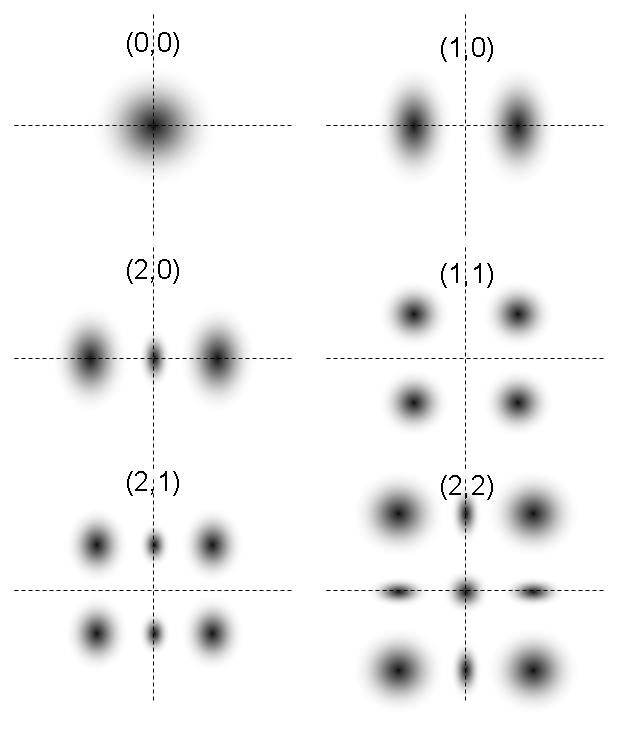
\includegraphics[width=5.5cm]{hermite/figures/gauss}
\caption{Some Gauss--Hermite modes.}
\label{fig-gauss-hermite}
\end{figure}

\begin{cue}
What was the relationship again between the Hermite polynomials and the Gauss-Hermite modes?  
\end{cue}

Remember, the Gauss-Hermite modes are essentially a Gaussian mode multiplied by Hermite polynomials in the $x$ and $y$ directions. Therefore, they are characterised by two integer indices, indicating the order of the Hermite polynomials for each direction.

\begin{cue}
Why are the higher-order Gauss-Hermite modes broader?  
\end{cue}

The higher-order Gauss-Hermite modes are broader because they get multiplied by Hermite polynomials which 'emphasise' the values away from the origin.

\pagebreak


\sectionugent{Series expansion using Hermite polynomials}

Just as we did with Bessel functions, we can use Hermite polynomials to expand a function in a series. In order to do that, we will need to establish the correct orthogonality relation between Hermite polynomials and normalise them.

Consider the following two differential equations:

\begin{equation}
\phi'' - 2 x \phi' + 2m \phi = 0 \label{eq-hermite-ortho-1}
\end{equation}
\begin{equation}
\psi'' - 2 x \psi' + 2n \psi = 0 \label{eq-hermite-ortho-2}
\end{equation}

The solutions of these are $H_m(x)$ and $H_n(x)$ respectively.

\begin{cue}
Multiplying Eq.~\ref{eq-hermite-ortho-1} by $\psi e^{-x^2}$, Eq.~\ref{eq-hermite-ortho-2} by $\phi e^{-x^2}$ and subtract the two equations.
\end{cue}

Performing these manipulations, we get

\begin{equation}
e^{-x^2}\left(\phi''\psi -\psi''\phi\right)- e^{-x^2} 2 x \left(\phi'\psi -\psi'\phi\right)+ e^{-x^2}2(m-n)\phi\psi = 0
\end{equation} 

\begin{cue}
Identify a total differential in the first terms of this equation.
\end{cue}

This can be written as

\begin{equation}
\left[e^{-x^2}\left(\phi'\psi -\psi'\phi\right)\right]' = e^{-x^2}2(n-m)\phi\psi
\end{equation} 

Integrating this between $-\infty$ and $\infty$ we get

\begin{equation}
2(n-m)\int_{-\infty}^{\infty}e^{-x^2}\phi\psi dx = \left[e^{-x^2}\left(\phi'\psi -\psi'\phi\right)\right]_{-\infty}^{+\infty}
\end{equation} 

The right hand side is equal to zero, because $e^{-{\infty}^2}$ goes to zero more quickly than any polynomial.

So in the end we get

\begin{equation}
\fbox{$\displaystyle
\int_{-\infty}^{\infty}e^{-x^2}H_n(x)H_m(x)dx = 0, \hspace{0.5cm} n \ne m \label{eq-hermite-ortho}
$}
\end{equation} 

This is the orthogonality relation for Hermite polynomials: they are orthogonal over the interval $[-\infty, \infty]$ with the weighting function $e^{-x^2}$.


To normalise the Hermite polynomials, we need to calculate

\begin{equation}
I = \int_{-\infty}^{\infty}e^{-x^2}H_n^2(x)dx
\end{equation}

\begin{cue}
Multiplying the generating function by itself and by $e^{-x^2}$. Careful: can you use $t$ in both copies of the generating function? Afterwards, integrate from $-\infty$ to $\infty$ and simplify. 
\end{cue}

We first multiply the generating function Eq.~\ref{eq-g-hermite} by itself and by $e^{-x^2}$:

\begin{equation}
e^{-x^2} e^{-t^2 + 2tx} e^{-s^2 + 2sx}= \sum_{m, n = 0}^{\infty}e^{-x^2} H_n(x)\frac{t^n}{n!}H_m(x)\frac{s^m}{m!}
\end{equation} 

When we integrate this over $x$ from $-\infty$ to $\infty$, the terms with $m \ne n$ on the right--hand side drop out because of the orthogonality relation Eq.~\ref{eq-hermite-ortho}:

\begin{equation}
\int_{-\infty}^{\infty} e^{-x^2} e^{-t^2 + 2tx} e^{-s^2 + 2sx} dx= \sum_{n = 0}^{\infty} \int_{-\infty}^{\infty} e^{-x^2} H_n^2(x)\frac{(st)^n}{n!n!} dx \label{eq-hermite-norm-1}
\end{equation}

\begin{exer}
% difficulty: hard
Show that $\int_{-\infty}^{\infty}e^{-x^2}dx = \sqrt{\pi}$
\begin{hnt}
Write the integral as
$$\sqrt{\int_{-\infty}^{\infty} e^{-x^2}dx\int_{-\infty}^{\infty} e^{-y^2}dy}$$
and transform it to polar coordinates with $x^2+y^2=r^2$ and $dxdy = r dr d\theta$.
\end{hnt}
\end{exer}

\begin{cue}
Using the result from the exercise above, evaluate the left--hand side of Eq.~\ref{eq-hermite-norm-1}.
\end{cue}

For the integral on the left--hand side of Eq.~\ref{eq-hermite-norm-1}, we get 

\begin{align}
\int_{-\infty}^{\infty} e^{-x^2} e^{-t^2 + 2tx} e^{-s^2 + 2sx} dx 
  = & \int_{-\infty}^{\infty} e^{-(x-s-t)^2} e^{2st}dx \nonumber \\
  = & \sqrt{\pi} e^{2st} \nonumber \\
  = & \sqrt{\pi} \sum_{n = 0}^{\infty} \frac{2^n{(st)}^n}{n!}  \label{eq-hermite-norm-2}
\end{align} 

\pagebreak

\begin{cue}
Compare the two different summations you derived so far to calculate the normalisation integral.
\end{cue}

By equating like powers of $st$ in the the right--hand sides of Eq.~\ref{eq-hermite-norm-1} and \ref{eq-hermite-norm-2}, we get the value of the normalisation integral:

\begin{equation}
\int_{-\infty}^{\infty} e^{-x^2} H_n^2(x) dx = 2^n n! \sqrt{\pi}
\end{equation} 

With this we can finally write the complete expression to expand a function $f(x)$ in a series of Hermite polynomials:

\begin{equation}
f(x) = \sum_{n=0}^{\infty}a_n H_n(x)
\end{equation} 

with

\begin{equation}
\fbox{$\displaystyle
a_n = \frac{1}{2^n n!\sqrt{\pi}} \int_{-\infty}^{\infty} e^{-x^2} H_n(x) f(x) dx
$}
\end{equation} 


\begin{exer}
% difficulty: trivial
% ugent
Prove the following parity relation:
$$H_n(x) = (-1)^nH_n(-x)$$
a) by using the series expansion of Hermite polynomials

b) by replacing $t$ by $-t$ and $x$ by $-x$ in the generating function
\end{exer}


\begin{exer}
% difficulty: normal
% ugent
Use the definition of the generating function for Hermite polynomials to prove that
$$H_{2n}(0) = (-1)^n \frac{(2n)!}{n!}$$
$$H_{2n+1}(0) = 0$$

How does this property translate to the Gauss-Hermite modes?

\end{exer}

\begin{marginfigure}[-16.0cm]
% credits: Wikipedia
% url: https://en.wikipedia.org/wiki/Olinde_Rodrigues
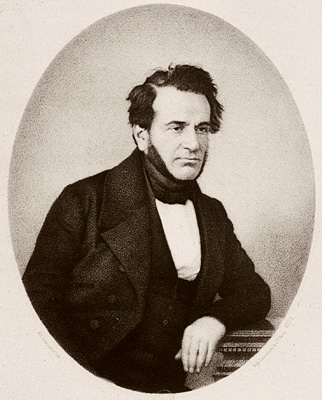
\includegraphics{hermite/figures/o_rodrigues}
\caption{Olinde Rodrigues (1795–1851)}
\end{marginfigure}

\begin{exer}
% difficulty: hard
% ugent  
Prove the Rodriguez formula for Hermite polynomials:
$$H_n(x) = (-1)^n e^{x^2}\frac{d^n}{d x^n}\left(e^{-x^2}\right)$$
\begin{hnt}
Verify this formula for a few values of $n$ to get a feeling for how it works, and then use mathematical induction.
\end{hnt}  
\end{exer}

\pagebreak

\begin{exer}
% difficulty: normal
For $0 \leq m \leq n-1$, use the Rodriguez formula to show that 
$$\int_{-\infty}^{\infty}x^m e^{-x^2} H_n(x) dx = 0$$
\end{exer}


\begin{exer}
% difficulty: normal 
Assume that based only on Hermite's differential equation, we managed to derive the recurrence relation involving $H_n'(x)$, as well as the values of $H_n(0)$. Based only on this information, derive the explicit form of the generating function $g(x,t)$ defined as

$$g(x,t) = \sum_{n = 0}^{\infty} H_n(x)\frac{t^n}{n!} $$

a) Take the derivative of $g(x,t)$ above with respect to $x$, use the recurrence relationship, and derive a first-order differential equation for $g(x,t)$.\\

b) Solve this equation to give

$$g(x,t) = e^{2tx} f(t)$$

c) Derive $f(t)$ by evaluating the expression for $x=0$.
\end{exer}

\begin{exer}
% difficulty: hard  
Prove that 
$$ | H_n(x) | \le  | H_n(jx) | $$
\begin{hnt}
  Remove factors from the series expansion of $ H_n(jx) $ so that it contains only positive terms.
\end{hnt}
\end{exer}


\begin{exer}
% difficulty: hard 
Show that 
$$\left( 2x - \frac{d}{dx} \right)^n 1 = H_n(x)$$
\begin{hnt}
  Verify this formula for a few values of $n$ to get a feeling for how it works, and then use mathematical induction.
\end{hnt}
\end{exer}


\begin{exer}
% difficulty: hard 
Calculate
$$ \int_{-\infty}^{\infty} e^{-x^2} x^2 H_n^2(x) dx $$
This integral occurs in the calculation of the mean-square displacement of a quantum oscillator.
\begin{sol}
$$ = 2^{n-1} (2n + 1) n! \sqrt{\pi}$$
\end{sol}
\begin{hnt}
Expand $x H_n(x)$ using a recurrence relation and apply the orthogonality conditions.
\end{hnt}  
\end{exer}

\pagebreak

\begin{exer}
% difficulty: hard  
Expand the following integral in a power series in $t$

$$ \int_{-\infty}^{\infty} e^{-x^2/2} g(x,t) dx$$

and use the result to calculate

$$\int_{-\infty}^{\infty} e^{-x^2/2} H_{m}(x) dx $$

\begin{sol}
$$\int_{-\infty}^{\infty} e^{-x^2/2} H_{2m}(x) dx = \frac{(2m)!}{m!} \sqrt{2\pi} $$
$$\int_{-\infty}^{\infty} e^{-x^2/2} H_{2m+1}(x) dx = 0 $$
\end{sol}
\end{exer}


\begin{exer}
% difficulty: hard  
Multiply the generating function by $t^{-k-1}$ and integrate over the unit circle in the complex $t$-plane to show that

$$H_k(x) =\frac{k!}{2 \pi j} \oint \frac{e^{-t^2 +2tx}}{t^{k+1}}dt $$

Then, show by direct substitution that this expression satisfies Hermite's differential equation.

\begin{hnt}
Try to write the integrand as a total differential.
\end{hnt}
  
\end{exer}


\section*{Review questions}

\begin{itemize}
\item What are Hermite polynomials functions?  
\item How can a generating function be used to define Hermite polynomials?
\item What is the relationship between Hermite polynomials and Gauss-Hermite modes?  
\item Under what scalar product are Hermite polynomials orthogonal?
\item For which physical systems would you use a series expansion based on Hermite polynomials?  
\end{itemize}



%%% Local Variables:
%%% mode: latex
%%% TeX-master: "../main"
%%% End:
